\documentclass[twocolumn]{article}
\usepackage{soul}
\usepackage{amsmath}
\usepackage[utf8]{inputenc}
\usepackage[left=2cm, right=2cm, top=50]{geometry}
\usepackage{multicol}
\setlength{\columnsep}{1cm}
\usepackage{graphicx}
\usepackage{subfigure}
\title{Ellipse}
\author{Diptasri Ghosh}
\date{EE21MTECH14004}
\usepackage{physics}

\usepackage{setspace}
\usepackage{gensymb}
\singlespacing
\usepackage{amsthm}
\usepackage{mathrsfs}
\usepackage{txfonts}
\usepackage{stfloats}
\usepackage{bm}
\usepackage{cite}
\usepackage{cases}
\usepackage{subfig}
\usepackage{longtable}
\usepackage{multirow}
\usepackage{enumitem}
\usepackage{mathtools}
\usepackage{steinmetz}
\usepackage{tikz}
\usepackage{circuitikz}
\usepackage{verbatim}
\usepackage{tfrupee}
\usepackage[breaklinks=true]{hyperref}
\usepackage{tkz-euclide}
\usetikzlibrary{calc,math}
\usepackage{listings}
    \usepackage{color}                                           
    \usepackage{array}                                            
    \usepackage{longtable}                                        
    \usepackage{calc}                                             
    \usepackage{multirow}                                         
    \usepackage{hhline}                                           
    \usepackage{ifthen} 
\usepackage{lscape}     
\usepackage{multicol}
\usepackage{chngcntr}
\DeclareMathOperator*{\Res}{Res}
\renewcommand\thesection{\arabic{section}}
\renewcommand\thesubsection{\thesection.\arabic{subsection}}
\renewcommand\thesubsubsection{\thesubsection.\arabic{subsubsection}}
\renewcommand\thesectiondis{\arabic{section}}
\renewcommand\thesubsectiondis{\thesectiondis.\arabic{subsection}}
\renewcommand\thesubsubsectiondis{\thesubsectiondis.\arabic{subsubsection}}
\hyphenation{op-tical net-works semi-conduc-tor}
\def\inputGnumericTable{}
\lstset{
%language=C,
frame=single, 
breaklines=true,
columns=fullflexible
}

\title{Straight Line}
\author{Diptasri Ghosh}
\date{EE21MTECH14004}



\newtheorem{theorem}{Theorem}[section]
\newtheorem{problem}{Problem}
\newtheorem{proposition}{Proposition}[section]
\newtheorem{lemma}{Lemma}[section]
\newtheorem{corollary}[theorem]{Corollary}
\newtheorem{example}{Example}[section]
\newtheorem{definition}[problem]{Definition}
\newcommand{\BEQA}{\begin{eqnarray}}
\newcommand{\EEQA}{\end{eqnarray}}
\newcommand{\define}{\stackrel{\triangle}{=}}
\bibliographystyle{IEEEtran}
\providecommand{\mbf}{\mathbf}
\providecommand{\pr}[1]{\ensuremath{\Pr\left(#1\right)}}
\providecommand{\qfunc}[1]{\ensuremath{Q\left(#1\right)}}
\providecommand{\sbrak}[1]{\ensuremath{{}\left[#1\right]}}
\providecommand{\lsbrak}[1]{\ensuremath{{}\left[#1\right.}}
\providecommand{\rsbrak}[1]{\ensuremath{{}\left.#1\right]}}
\providecommand{\brak}[1]{\ensuremath{\left(#1\right)}}
\providecommand{\lbrak}[1]{\ensuremath{\left(#1\right.}}
\providecommand{\rbrak}[1]{\ensuremath{\left.#1\right)}}
\providecommand{\cbrak}[1]{\ensuremath{\left\{#1\right\}}}
\providecommand{\lcbrak}[1]{\ensuremath{\left\{#1\right.}}
\providecommand{\rcbrak}[1]{\ensuremath{\left.#1\right\}}}
\theoremstyle{remark}
\newtheorem{rem}{Remark}
\newcommand{\sgn}{\mathop{\mathrm{sgn}}}
\providecommand{\abs}[1]{\left\vert#1\right\vert}
\providecommand{\res}[1]{\Res\displaylimits_{#1}} 
\providecommand{\norm}[1]{\left\lVert#1\right\rVert}
%\providecommand{\norm}[1]{\lVert#1\rVert}
\providecommand{\mtx}[1]{\mathbf{#1}}
\providecommand{\mean}[1]{E\left[ #1 \right]}
\providecommand{\fourier}{\overset{\mathcal{F}}{ \rightleftharpoons}}
%\providecommand{\hilbert}{\overset{\mathcal{H}}{ \rightleftharpoons}}
\providecommand{\system}{\overset{\mathcal{H}}{ \longleftrightarrow}}
	%\newcommand{\solution}[2]{\textbf{Solution:}{#1}}
\newcommand{\solution}{\noindent \textbf{Solution: }}
\newcommand{\cosec}{\,\text{cosec}\,}
\providecommand{\dec}[2]{\ensuremath{\overset{#1}{\underset{#2}{\gtrless}}}}
\newcommand{\myvec}[1]{\ensuremath{\begin{pmatrix}#1\end{pmatrix}}}
\newcommand{\mydet}[1]{\ensuremath{\begin{vmatrix}#1\end{vmatrix}}}
%\numberwithin{equation}{section}
\numberwithin{equation}{subsection}
%\numberwithin{problem}{section}
%\numberwithin{definition}{section}
\makeatletter
\@addtoreset{figure}{problem}
\makeatother
\let\StandardTheFigure\thefigure
\let\vec\mathbf
%\renewcommand{\thefigure}{\theproblem.\arabic{figure}}
\renewcommand{\thefigure}{\theproblem}
%\setlist[enumerate,1]{before=\renewcommand\theequation{\theenumi.\arabic{equation}}
%\counterwithin{equation}{enumi}
%\renewcommand{\theequation}{\arabic{subsection}.\arabic{equation}}
\def\putbox#1#2#3{\makebox[0in][l]{\makebox[#1][l]{}\raisebox{\baselineskip}[0in][0in]{\raisebox{#2}[0in][0in]{#3}}}}
     \def\rightbox#1{\makebox[0in][r]{#1}}
     \def\centbox#1{\makebox[0in]{#1}}
     \def\topbox#1{\raisebox{-\baselineskip}[0in][0in]{#1}}
     \def\midbox#1{\raisebox{-0.5\baselineskip}[0in][0in]{#1}}
\vspace{3cm}





\begin{document}

\maketitle
\textbf{\textit{Abstract} - This document contains solution of sketching loci of the given equation.}\\
\begin{center}
\textbf{\ul{Problem}}\\
Vector-2, Example-4, Question No.-7
\end{center}

\textbf{Question 7. Sketch the loci of the following equation}\\
\begin{align}
\frac{x^2}{4} + \frac{y^2}{9} = 1
\end{align}
\textbf{Solution :}\\
Given equation is,
\begin{align} \label{Eq a}
\frac{x^2}{4} + \frac{y^2}{9} = 1
\end{align} 
We can write equation (\ref{Eq a}) as,
\begin{align} \label{Eq b}
9 x^2 + 4 y^2 - 36 = 0
\end{align}
The general equation is given as,
\begin{align} \label{Eq c}
\textbf{x}^\top \textbf{V} \textbf{x} + 2 \textbf{u}^\top \textbf{x} + f = 0 
\end{align}
Comparing (\ref{Eq b}) and (\ref{Eq c}) we get,
\begin{align}
\vec{V}=\myvec{9 & 0 \\ 0 & 4} , \vec{u}=\myvec{0 \\ 0} , f = -36
\end{align}
The vertex of ellipse is given as \textbf{c} and can be obtained from,
\begin{align} \label{Eq d}
\textbf{c} = - \textbf{V}^-^1 \textbf{u}
\end{align}
We know,
\begin{align}
\textbf{V}^-^1 = \frac{1}{\begin{vmatrix}\textbf{V}\end{vmatrix}} Adj \textbf{V}
\end{align}
Putting the values of \begin{vmatrix}\textbf{V}\end{vmatrix} and Adj \textbf{V} we get,
\begin{align}
\textbf{V}^-^1 = \frac{1}{36} \myvec{4 & 0 \\ 0 & 9}^\top   
 = \myvec{\dfrac{4}{36} & 0 \\ 0 & \dfrac{9}{36}} 
\end{align}
Putting values in equation (\ref{Eq d}) we get the vertex of the ellipse,
\begin{align}
\vec{c}=\myvec{0 \\ 0}
\end{align}
The length of semi major axis and semi minor axis are given by,
\begin{align} \label{Eq e}
\sqrt{\frac{\textbf{u}^\top \textbf{V}^-^1 \textbf{u} - f}{ \lambda_1}} = 3   ,   \sqrt{\frac{\textbf{u}^\top \textbf{V}^-^1 \textbf{u} - f}{ \lambda_2}} = 2
 \end{align}
Solving equation (\ref{Eq e}) we get,
\begin{align} 
\lambda_1 = 4   ,   \lambda_2 = 9
\end{align}
The eccentricity of ellipse is given by,
\begin{align} \label{Eq f}
e = \sqrt{1 - \frac{\lambda_1}{\lambda_2}}
\end{align}
Putting the values in equation (\ref{Eq f}) we get,
\begin{align}
e = \frac{\sqrt{5}}{3}
\end{align}
The directrices of ellipse is given by,
\begin{align} \label{Eq g}
c = \frac{e \textbf{u}^\top \textbf{n} \pm \sqrt{e^2 (\textbf{u}^\top n)^2 - \lambda_2 (e^2 - 1) (||\textbf{u}||^2 - \lambda_2 f)}}{\lambda_2 e (e^2 - 1)}
\end{align}
Where
\begin{align}
\vec{n} = \sqrt{\lambda_2} \textbf p_1 = \myvec{0 \\ 1}
\end{align}
As
\begin{align}
 \vec{p_1} = \frac{1}{\sqrt{9}} \myvec{0 \\ 1}
\end{align}
Putting the values in equation (\ref{Eq g}) we get directrices of the ellipse,
\begin{align}
c = \pm \frac{9}{\sqrt{5}}
\end{align}
The foci of ellipse is given by,
\begin{align} \label{Eq h}
\textbf{F} = \frac{c e^2 \textbf{n} - \textbf{u}}{\lambda_2}
\end{align}
Putting the respective values in equation (\ref{Eq h}) we get,
\begin{align}
\vec{F}=\myvec{0 \\ \dfrac{\sqrt{5}}{3}}
\end{align}

\begin{figure}[!ht]
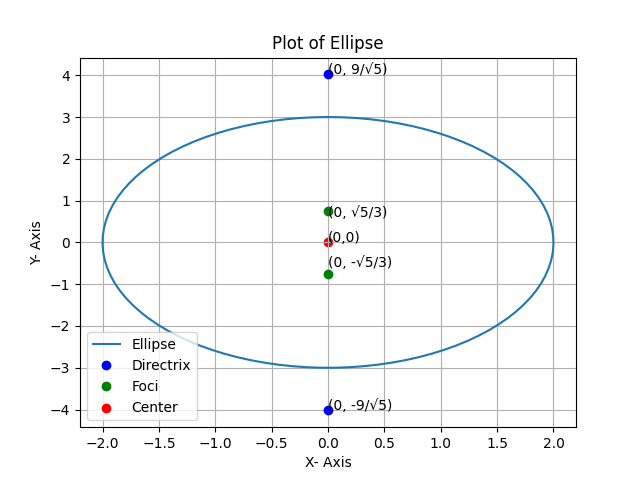
\includegraphics[width=1.1\columnwidth]{Figure_1.png}
\caption{Plot of the Ellipse with vertex \vec{c}=\myvec{0 \\ 0}}
\label{fig}
\end{figure}
\end{document}



